% !Mode:: "TeX:UTF-8"
% !TEX program  = xelatex
\documentclass[a4paper]{article}
\usepackage{amsmath}
\usepackage{amssymb}
\usepackage{ctex}
\usepackage{graphicx}
%\usepackage{braket}
\usepackage[european]{circuitikz}
\usepackage{multirow}
\usepackage{geometry}
\usepackage{float}
\geometry{left=2.5cm,right=2.5cm,bottom=2.5cm,top=2.5cm}
\title{物理化学拓展实验: 电导率测定氯化银解离平衡反应热力学常数}
\author{薛明怡\quad 151250177\quad 化学化工学院}
\date{\today}
\begin{document}
\maketitle
%%\tableofcontents
%%\bibliographystyle{unsrt}
\section{实验目的}
\begin{enumerate}
	\item 掌握电导法测定电解质溶液的摩尔电导.
	\item 了解电导率的应用.
\end{enumerate}
\section{实验原理}
\subsection{电导率}
电导率是电阻率($\rho$)的倒数, 是衡量物质导电能力的基本性质, 通常用希腊字母$\sigma$表示.
\begin{equation}
	\centering
	\begin{aligned}
		\rho &= R\frac{A}{l}\\
		\kappa &= \frac{1}{\rho}= G\frac{l}{A}\\
	\end{aligned}
\end{equation}
\begin{figure}[H]
	\centering
	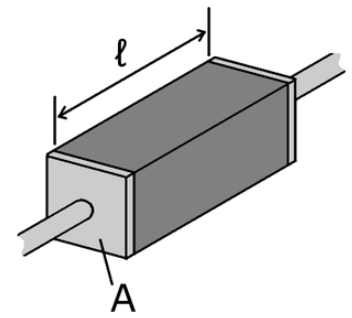
\includegraphics[width=0.2\paperwidth]{fig/resistivity_conductivity_definition.PNG}
	\caption{电阻率和电导率的定义}
\end{figure}
其中, $R$是均匀样品的电阻, $l$是样品的长度, $A$是样品截面面积.
电阻率的单位是$\Omega\cdot m$, 电导率的单位是$S/m$.
\par
更一般的标量定义方式是,
\begin{equation}
	\centering
	\begin{aligned}
		\rho &= \frac{E}{J}\\
		\kappa &= \frac{1}{\rho} = \frac{J}{E}\\
	\end{aligned}
\end{equation}
其中, $E$是电场强度, $J$是电流密度. 例如, 
橡胶是一种具有高电阻率低电导率的材料, 因为将橡胶放置
在强电场中几乎不产生电流. 相反, 铜是一种具有低电阻率高电导率
的材料, 因为即使一个小的电场也能产生大的电流通过.
\par
上述定义很自然的可以导出电阻率和电导率的张量定义, 
张量定义是一种完全广义的定义方式, 但由于定义最为复杂因此只在各向异性
情景中被使用. 如果材料不是各向异性的, 用上述两种简单的表达式即可. 
如石墨在微观上由一层层的石墨烯构成, 电流可以轻易的在每一层上通过, 
但是无法轻易的从一层流到与它相邻的另一层. 在后面的情景下, 
电流的流向不完全与电场方向一致, 从而需要使用电导率的张量定义.
\begin{equation}
	\centering
	\begin{aligned}
		\mathbf{J} &= \mathbf{\kappa} \mathbf{E}\\
		\left[\begin{matrix}
			J_{x}\\
			J_{y}\\
			J_{z}\\ 
	  \end{matrix}\right]
	  &=
		\left[\begin{matrix}
			\kappa_{xx} & \kappa_{xy} & \kappa_{xz} \\
			\kappa_{yx} & \kappa_{yy} & \kappa_{yz} \\
			\kappa_{zx} & \kappa_{zy} & \kappa_{zz} 
		\end{matrix}\right] 
		\left[\begin{matrix}
			  E_{x}\\
			  E_{y}\\
			  E_{z}\\ 
		\end{matrix}\right]
	\end{aligned}
\end{equation}
\subsection{摩尔电导率}
摩尔电导率$\Lambda_{m}$是指把含有$1mol$电解质的溶液置于相距为单位距离
的电导池的两个平行电极之间, 这时所具有的电导. 由于对不同的电解质均取$1mol$
但所取溶液的体积$V_{m}$将随浓度而改变. 设$c$是电解质溶液的浓度(单位为$mol\cdot m^{-3}$), 
则含$1mol$电解质的溶液的体积$V_{m}$应等于$\frac{1}{c}$, 根据电导率$\kappa$的定义, 
摩尔电导率$\Lambda_{m}$,
\begin{equation}
	\Lambda_{m} = \kappa V_{m} = \frac{\kappa}{c}\\
\end{equation}
% \subsection{电导池常数}
% 电导池中两极之间的距离$l$和涂有波黑的电极面积$A$是很难测量的, 通常是把已知电阻率的溶液
% (通常是一定浓度的$KCl$溶液)注入电导池, 就可确定$\frac{l}{A}$值, 这个值被称为电导池常数
% $K_{cell}$,
% \begin{equation}
% 	K_{cell} = \frac{1}{\rho}R = \kappa R\\
% \end{equation}
\subsection{氯化银的溶解平衡与溶度积}
$AgCl$为难溶盐, 在水中溶解度小导致浓度无法用普通的滴定法测定, 但可以用电导法求得. 
首先先制备饱和$AgCl$溶液, 测量溶液的电导率$\kappa(solution)$,
\begin{equation}
	\kappa(AgCl) = \kappa(solution) - \kappa(H_{2}O)\\
\end{equation}
摩尔电导率的计算公式为,
\begin{equation}
	\Lambda_{m}(AgCl) = \frac{\kappa(AgCl)}{c(AgCl)}\\
\end{equation}
由于难溶盐的溶解度很小, 溶液极稀, 所以可以认为$\Lambda_{m} \approx \Lambda_{m}^{\infty}$, 
而$\Lambda_{m}^{\infty}$的值可以由离子无限稀释摩尔电导率相加而得, 
\begin{equation}
	\Lambda_{m}^{\infty}(AgCl) = 	\Lambda_{m}^{\infty}(Ag^{+}) +	\Lambda_{m}^{\infty}(Cl^{-})\\
\end{equation}
由式(6)可以求得饱和$AgCl$溶液的浓度, 
\begin{equation}
	\centering
	\begin{aligned}
		c(AgCl) &= \frac{\kappa(AgCl)}{\Lambda_{m}(AgCl)}\\
				&=\frac{\kappa(AgCl)}{\Lambda_{m}^{\infty}(AgCl)}\\
				&=\frac{\kappa(AgCl)}{\Lambda_{m}^{\infty}(Ag^{+}) +	\Lambda_{m}^{\infty}(Cl^{-})}\\
	\end{aligned}
\end{equation}
最后根据下式可以得到$AgCl$的溶度积.
\begin{equation}
	\centering
	\begin{aligned}
		K_{sp} &= a_{Ag^{+}} \cdot a_{Cl^{-}}\\
		&= \gamma_{\pm}^{2} \cdot 
		\frac{c_{Ag^{+}} c_{Cl^{-}}}{C^{\theta 2}} \\
		&\approx \frac{c_{Ag^{+}} c_{Cl^{-}}}{c_{\theta}^{2}} \\
		&=(\frac{c_{AgCl}}{c_{\theta}})^{2}\\
	\end{aligned}
\end{equation}
\subsection{解离平衡热力学常数}
氯化银解离平衡反应如下, 
\begin{equation}
	AgCl \to Ag^{+} + Cl^{-}
\end{equation}
假定在温度变化范围不大的情况下, 标准摩尔焓和标准摩尔熵可以视为常数, 
因此$lnK_{sp}$与$\frac{1}{T}$成一次函数关系, 并可求得在$298.15K$时
解离平衡的标准摩尔吉布斯自由能.
\begin{equation}
	\centering
	\begin{aligned}
		\Delta_{r}G_{m}^{\theta} &= -RTlnK_{sp}\\
		&=\Delta_{r}H_{m}^{\theta} + T\Delta_{r}S_{m}^{\theta}\\
		lnK_{sp} &= -\frac{\Delta_{r}H_{m}^{\theta}}{RT} - \frac{\Delta_{r}S_{m}^{\theta}}{R}\\
	\end{aligned}
\end{equation}
\section{仪器与药品}
\begin{enumerate}
    \item \textbf{仪器:} 电导率仪, 恒温槽, 吸滤瓶, $50mL$烧杯
    \item \textbf{药品:} $0.1mol/L~AgNO_{3}$溶液, $0.1mol/L~KCl$溶液, 电导水
\end{enumerate}
\section{实验步骤}
\subsection{$AgCl$的制备}
\begin{itemize}
	\item 取$10mL$ $0.1mol/L~AgNO_{3}$溶液于烧杯中, 
	向其中加入$10mL$ $0.1mol/L~KCl$溶液(边加边搅拌).
	\item 用吸滤瓶过滤溶液, 滴加电导水抽滤3次. 
	\item 称量制得的白色固体, 并将其保存在棕色试剂瓶中或立即使用.
\end{itemize}
\subsection{测定饱和$AgCl$溶液电导率}
\begin{itemize}
	\item 取少量新制的$AgCl$固体溶解在$50mL$烧杯中, 加入$20mL$电导水, 
	搅拌, 在$25^\circ$C恒温槽中静置约$30min$, 达到溶解平衡.
	\item 测定该温度下饱和$AgCl$溶液和电导水的电导率. 
	\item 重复上述步骤, 继续测定$30^\circ$C, $35^\circ$C, $40^\circ$C, 
	$50^\circ$C下饱和$AgCl$溶液和电导水的电导率.
	\item 用电导法测量的$AgCl$溶度积可与电动势测定实验中的值进行对比.
\end{itemize}
\newpage
\section{数据处理}


\newpage
\section{原始数据记录}
\begin{table}[H]
	\caption{电导率测定实验数据}
	\begin{center}
		\begin{tabular}{l|l|l}
			\hline
			温度/$^\circ$C \quad\quad\quad\quad\quad 	&饱和$AgCl$溶液电导率$\kappa$/$S\cdot m^{-1}$\quad\quad\quad\quad\quad & 电导水电导率$\kappa_{0}$/$S\cdot m^{-1}$\\
			\hline
			25&&\\
			&&\\
			\hline
			30&&\\
			&&\\
			\hline
			35&&\\
			&&\\
			\hline
			40&&\\
			&&\\
			\hline
			50&&\\
			&&\\
			\hline
		 \end{tabular}
	\end{center}
\end{table}
%%\bibliography{ref}
\end{document}